% ----- auto-generated from week_04/Week*.html via pandoc -----
\chapter{Adaptive Control (Week 4)}
\labch{week_04}



Lyapunov-Based Adaptive Control for Robotic Systems with Parametric Uncertainty

M.Sc. Control for Robots --- AY 2025--26\\
3-Hour Lecture \& Lab • Week 4 of 12

\section{Overview}

\subsection{Week 3 Recall --- Model Predictive Control --- Exam Practice}

Before we begin new material, spend 20 minutes working through these two exam-style questions that cover last week\textquotesingle s MPC content. Write your solutions on paper.

\subsubsection{Question 1 --- MPC Problem Formulation \& Lifted Form (10 marks)}

Consider a discrete-time linear time-invariant system:

\[
                    x_{k+1} = A\,x_k + B\,u_k
                \]

with state \(x_k \in \mathbb{R}^n\), control \(u_k \in \mathbb{R}^m\), and a finite prediction horizon \(N\). The MPC cost function is:

\[
                    J = \sum_{i=0}^{N-1}\Big[\big(x_{k+i} - x_{\mathrm{ref}}\big)^T Q \big(x_{k+i} - x_{\mathrm{ref}}\big) + u_{k+i}^T R\, u_{k+i}\Big]
                \]

where \(Q \succeq 0\) and \(R \succ 0\).

\textbf{(a)} By recursive substitution, show that the predicted state sequence can be written in compact (lifted) form as:

\[
                    \mathbf{X} = \mathcal{A}\,x_k + \mathcal{B}\,\mathbf{U}
                \]

where the stacked vectors are \(\mathbf{X} = \begin{bmatrix} x_{k+1} \\ x_{k+2} \\ \vdots \\ x_{k+N} \end{bmatrix}\) and \(\mathbf{U} = \begin{bmatrix} u_k \\ u_{k+1} \\ \vdots \\ u_{k+N-1} \end{bmatrix}\), and derive the explicit forms:

\[
                    \mathcal{A} = \begin{bmatrix} A \\ A^2 \\ A^3 \\ \vdots \\ A^N \end{bmatrix}, \qquad
                    \mathcal{B} = \begin{bmatrix}
                        B & 0 & 0 & \cdots & 0 \\
                        AB & B & 0 & \cdots & 0 \\
                        A^2B & AB & B & \cdots & 0 \\
                        \vdots & \vdots & \vdots & \ddots & \vdots \\
                        A^{N-1}B & A^{N-2}B & A^{N-3}B & \cdots & B
                    \end{bmatrix}
                \]

Show every substitution step from \(i=1\) to \(i=N\).

\textbf{(b)} Identify the structure of \(\mathcal{B}\) (lower-triangular block Toeplitz). Explain why this structure arises from the causal nature of the system (future states depend only on past and present inputs).

\subsubsection{Question 2 --- Deriving the Optimal MPC Control Law (10 marks)}

Starting from the lifted quadratic cost:

\[
                    J = \big(\mathbf{X} - \mathbf{X}_{\mathrm{ref}}\big)^T \bar{Q}\,\big(\mathbf{X} - \mathbf{X}_{\mathrm{ref}}\big) + \mathbf{U}^T \bar{R}\,\mathbf{U}
                \]

where \(\bar{Q} = \mathrm{blkdiag}(Q, Q, \dots, Q) \in \mathbb{R}^{nN \times nN}\) and \(\bar{R} = \mathrm{blkdiag}(R, R, \dots, R) \in \mathbb{R}^{mN \times mN}\):

\textbf{(a)} Substitute \(\mathbf{X} = \mathcal{A}\,x_k + \mathcal{B}\,\mathbf{U}\) into \(J\) and expand fully:

\[
                    J = \big(\mathcal{A}\,x_k + \mathcal{B}\,\mathbf{U} - \mathbf{X}_{\mathrm{ref}}\big)^T \bar{Q}\,\big(\mathcal{A}\,x_k + \mathcal{B}\,\mathbf{U} - \mathbf{X}_{\mathrm{ref}}\big) + \mathbf{U}^T \bar{R}\,\mathbf{U}
                \]

Let \(\mathbf{E} = \mathbf{X}_{\mathrm{ref}} - \mathcal{A}\,x_k\). Show that:

\[
                    J = \mathbf{U}^T\!\big(\mathcal{B}^T \bar{Q}\,\mathcal{B} + \bar{R}\big)\mathbf{U} - 2\,\mathbf{E}^T \bar{Q}\,\mathcal{B}\,\mathbf{U} + \mathbf{E}^T \bar{Q}\,\mathbf{E}
                \]

\textbf{(b)} Take \(\frac{\partial J}{\partial \mathbf{U}} = 0\) and derive:

\[
                    \mathbf{U}^* = \big(\mathcal{B}^T \bar{Q}\,\mathcal{B} + \bar{R}\big)^{-1} \mathcal{B}^T \bar{Q}\,\big(\mathbf{X}_{\mathrm{ref}} - \mathcal{A}\,x_k\big)
                \]

\textbf{(c)} Define the MPC gain. Since only the first \(m\) rows of \(\mathbf{U}^*\) are applied (receding horizon), let \(E_1 = [I_m \;\; 0 \;\; \cdots \;\; 0]\). Then:

\[
                    u_k^* = E_1 \mathbf{U}^* = \underset{\text{\footnotesize K_{\mathrm{MPC,ref}}}}{\underline{E_1 \big(\mathcal{B}^T \bar{Q}\,\mathcal{B} + \bar{R}\big)^{-1} \mathcal{B}^T \bar{Q}}}\,\mathbf{X}_{\mathrm{ref}} - \underset{\text{\footnotesize K_{\mathrm{MPC}}}}{\underline{E_1 \big(\mathcal{B}^T \bar{Q}\,\mathcal{B} + \bar{R}\big)^{-1} \mathcal{B}^T \bar{Q}\,\mathcal{A}}}\,x_k
                \]

Explain why \(K_{\mathrm{MPC}}\) is a state-feedback gain and how increasing \(R\) relative to \(Q\) affects the control aggressiveness.

\textbf{Time limit: 20 minutes.} This is exactly the format and difficulty level you will encounter in the final exam. Write full derivations showing every step. Partial credit is awarded for correct intermediate work.

\subsection{Learning Outcomes}

\begin{itemize}
\tightlist
\item
  Understand why adaptive control is needed when system parameters are unknown or time-varying, and articulate the limitations of computed torque and MPC that assume known models.
\item
  Derive the adaptive control law using Lyapunov-based stability analysis, including the construction of a candidate Lyapunov function and verification that its time derivative is negative semi-definite.
\item
  Apply the linearity-in-parameters property of rigid-body dynamics: \(M(q)\ddot{q} + C(q,\dot{q})\dot{q} + G(q) = Y(q, \dot{q}, \ddot{q})\,\theta\), identifying the regressor matrix \(Y\) and parameter vector \(\theta\) for specific systems.
\item
  Implement adaptive control for three robotic platforms: a 2-DOF manipulator, a differential-drive mobile robot, and a quadrotor UAV.
\item
  Simulate and compare the performance of fixed-model computed torque control versus adaptive control under parameter uncertainty, demonstrating convergence of parameter estimates.
\end{itemize}

\section{Adaptive Control Theory}

\subsection{Why Adaptive Control?}

In Week 1, we designed a computed torque controller for a 2-DOF manipulator. The control law was:

\[
                \tau = M(q)\big(\ddot{q}_d + K_v\dot{e} + K_p e\big) + C(q,\dot{q})\dot{q} + G(q)
            \]

This requires \textbf{exact knowledge} of the inertia matrix \(M(q)\), Coriolis/centrifugal matrix \(C(q,\dot{q})\), and gravity vector \(G(q)\). In practice, this assumption fails for several reasons:

\begin{itemize}
\tightlist
\item
  \textbf{Unknown payloads:} A manipulator picks up objects of unknown mass. The effective \(m_2\) changes.
\item
  \textbf{Manufacturing tolerances:} Link lengths, masses, and centres of gravity are only approximately known.
\item
  \textbf{Wear and degradation:} Friction coefficients, gear ratios, and joint stiffness change over time.
\item
  \textbf{Model simplification:} We ignore link flexibility, actuator dynamics, and higher-order effects.
\end{itemize}

\textbf{Key insight:} If the model parameters used in computed torque are wrong, the nonlinear cancellation is imperfect, and the closed-loop system is no longer a simple linear error system. Tracking performance degrades, and stability may be lost.

Adaptive control addresses this by estimating the unknown parameters online, while simultaneously controlling the system. The parameter estimates converge to values that ensure good tracking, even if the true parameters are never exactly identified.

\textbf{Figure 1:} Adaptive control block diagram. The {blue control loop} tracks the reference, while the {orange adaptation loop} estimates unknown plant parameters and feeds them to the controller.

\textbf{Figure 2:} Comparison of {Direct} and {Indirect} adaptive control. In direct adaptation, the error signal is fed to an adaptation law that adjusts controller gains K(t) directly. In indirect adaptation, the error drives a parameter estimator to obtain θ̂, which is then used in a gain computation step to determine K(θ̂).

\subsection{The Linearity-in-Parameters Property}

The dynamics of a rigid-body robotic system can always be written as:

\(M(q)\ddot{q} + C(q,\dot{q})\dot{q} + G(q) = Y(q, \dot{q}, \ddot{q})\,\theta\)

where:

\begin{itemize}
\tightlist
\item
  \(Y(q, \dot{q}, \ddot{q}) \in \mathbb{R}^{n \times p}\) is the \textbf{regressor matrix} --- a known matrix that depends on joint positions, velocities, and accelerations, but \emph{not} on the unknown parameters.
\item
  \(\theta \in \mathbb{R}^p\) is the \textbf{parameter vector} --- a constant vector containing all the unknown dynamic parameters (products of masses, lengths, inertias, friction coefficients, etc.).
\end{itemize}

This is the \emph{linearity-in-parameters} property. It holds because the equations of motion are derived from the Lagrangian, which is quadratic in velocities and linear in the inertial parameters. The property is fundamental to adaptive control: it allows us to separate what we know (the structure of \(Y\)) from what we do not know (the values in \(\theta\)).

\textbf{Figure 3:} The linearity-in-parameters property separates robot dynamics into a {known regressor matrix Y} (computable from kinematics) multiplied by an {unknown parameter vector θ} (to be estimated online).

\subsection{Concrete Example: 2-DOF Planar Manipulator}

\textbf{Figure 4:} 2-DOF planar manipulator. {Link 1} (length l₁, mass m₁) and {Link 2} (length l₂, mass m₂) rotate at joints with angles θ₁ and θ₂. Joint torques τ₁ and τ₂ are the control inputs.

Consider the 2-DOF planar manipulator with link masses \(m_1, m_2\), link lengths \(l_1, l_2\), and gravity \(g\). The standard Euler-Lagrange dynamics are:

\[
                M(q)\ddot{q} + C(q,\dot{q})\dot{q} + G(q) = \tau
            \]

with:

\[
                M(q) = \begin{bmatrix}
                    m_1 l_1^2 + m_2(l_1^2 + l_2^2 + 2l_1 l_2 \cos q_2) & m_2(l_2^2 + l_1 l_2 \cos q_2) \\
                    m_2(l_2^2 + l_1 l_2 \cos q_2) & m_2 l_2^2
                \end{bmatrix}
            \]
\[
                C(q,\dot{q}) = \begin{bmatrix}
                    -m_2 l_1 l_2 \sin(q_2)\,\dot{q}_2 & -m_2 l_1 l_2 \sin(q_2)(\dot{q}_1 + \dot{q}_2) \\
                    m_2 l_1 l_2 \sin(q_2)\,\dot{q}_1 & 0
                \end{bmatrix}
            \]
\[
                G(q) = \begin{bmatrix}
                    (m_1 + m_2)\,g\,l_1 \sin q_1 + m_2\,g\,l_2 \sin(q_1 + q_2) \\
                    m_2\,g\,l_2 \sin(q_1 + q_2)
                \end{bmatrix}
            \]

Define the parameter vector:

\[
                    \theta = \begin{bmatrix} \theta_1 \\ \theta_2 \\ \theta_3 \\ \theta_4 \\ \theta_5 \\ \theta_6 \end{bmatrix}
                    = \begin{bmatrix} m_1 l_1^2 \\ m_2 l_1^2 \\ m_2 l_2^2 \\ m_2 l_1 l_2 \\ (m_1 + m_2)\,g\,l_1 \\ m_2\,g\,l_2 \end{bmatrix}
                \]

Then the regressor matrix \(Y \in \mathbb{R}^{2 \times 6}\) such that \(\tau = Y(q, \dot{q}, \ddot{q})\,\theta\) is:

\[
                    Y = \begin{bmatrix}
                        \ddot{q}_1 & \ddot{q}_1 & \ddot{q}_1 + \ddot{q}_2 & 2\cos(q_2)\ddot{q}_1 + \cos(q_2)\ddot{q}_2 - \sin(q_2)\dot{q}_2\dot{q}_1 - \sin(q_2)(\dot{q}_1+\dot{q}_2)\dot{q}_2 & \sin(q_1) & \sin(q_1+q_2) \\
                        0 & 0 & \ddot{q}_1 + \ddot{q}_2 & \cos(q_2)\ddot{q}_1 + \sin(q_2)\dot{q}_1^2 & 0 & \sin(q_1+q_2)
                    \end{bmatrix}
                \]

You can verify: multiply \(Y\theta\) and recover exactly \(M(q)\ddot{q} + C(q,\dot{q})\dot{q} + G(q)\). Every entry of \(Y\) is computable from measured (or commanded) \(q, \dot{q}, \ddot{q}\).

\subsection{The Adaptive Control Law}

We now construct the adaptive controller. Define the tracking error and its filtered version:

\[
                    e = q_d - q, \qquad \dot{e} = \dot{q}_d - \dot{q}
                \]

Define the \textbf{sliding variable} (composite error):

\[
                    s = \dot{e} + \Lambda\, e
                \]

where \(\Lambda = \Lambda^T \succ 0\) is a positive definite design matrix. Equivalently, define the \textbf{reference velocity} and \textbf{reference acceleration}:

\[
                \dot{q}_r = \dot{q}_d + \Lambda\,e = \dot{q} + s
            \]
\[
                \ddot{q}_r = \ddot{q}_d + \Lambda\,\dot{e}
            \]

Notice that \(s = \dot{q}_r - \dot{q}\), so \(s \to 0\) implies \(\dot{q} \to \dot{q}_r\), which combined with the definition of \(\dot{q}_r\) implies both \(e \to 0\) and \(\dot{e} \to 0\) exponentially (since \(\dot{e} + \Lambda e = 0\) is a stable linear ODE).

The \textbf{adaptive control law} is:

\(\tau = Y(q, \dot{q}, \dot{q}_r, \ddot{q}_r)\,\hat{\theta} + K_D\, s\)

where:

\begin{itemize}
\tightlist
\item
  \(\hat{\theta}\) is the current estimate of the parameter vector \(\theta\).
\item
  \(Y(q, \dot{q}, \dot{q}_r, \ddot{q}_r)\) is the regressor evaluated at the \emph{reference} velocity and acceleration (not the actual \(\ddot{q}\), which we cannot measure cleanly).
\item
  \(K_D = K_D^T \succ 0\) is a positive definite gain matrix providing damping on the sliding variable.
\end{itemize}

\textbf{Important subtlety:} We evaluate the regressor at \((\dot{q}_r, \ddot{q}_r)\) instead of \((\dot{q}, \ddot{q})\). This avoids the need to measure or numerically differentiate joint accelerations, and it ensures that the regressor is known (computable from \(q, \dot{q}, q_d, \dot{q}_d, \ddot{q}_d\)).

\subsection{Parameter Update Law}

The parameter estimates are updated according to:

\(\dot{\hat{\theta}} = \Gamma^{-1}\, Y^T\! s\)

where \(\Gamma = \Gamma^T \succ 0\) is the \textbf{adaptation gain matrix}. Define the parameter estimation error:

\[
                \tilde{\theta} = \hat{\theta} - \theta
            \]

Since \(\theta\) is constant, \(\dot{\tilde{\theta}} = \dot{\hat{\theta}}\).

\textbf{Figure 8:} Parameter convergence under adaptive control. Multiple parameter estimates starting from different initial conditions all converge toward the true parameter value θ* (dashed line). The adaptation law drives estimates toward values that minimize tracking error.

\subsection{Lyapunov Stability Proof}

\subsubsection{Theorem (Adaptive Control Stability)}

Under the adaptive control law \(\tau = Y\hat{\theta} + K_D s\) with the update law \(\dot{\hat{\theta}} = \Gamma^{-1} Y^T s\), the sliding variable \(s \to 0\) and consequently the tracking errors \(e \to 0\), \(\dot{e} \to 0\) as \(t \to \infty\).

\textbf{Figure 7:} Lyapunov stability concept. Left: the Lyapunov function V forms a bowl-shaped surface, and the system trajectory (pink spiral) descends toward the equilibrium. Right: V(t) monotonically decreases over time since V̇ = -sᵀK₄s is always non-positive.

\textbf{Proof.} Define the candidate Lyapunov function:

\[
                V = \frac{1}{2}\,s^T M(q)\,s + \frac{1}{2}\,\tilde{\theta}^T \Gamma\,\tilde{\theta}
            \]

Since \(M(q) \succ 0\) and \(\Gamma \succ 0\), both terms are strictly positive for \((s, \tilde{\theta}) \neq (0,0)\), so \(V\) is a valid positive definite candidate with \(V = 0\) iff \(s = 0\) and \(\tilde{\theta} = 0\).

\textbf{Step 1: Time derivative of \(V\).}

\[
                \dot{V} = s^T M(q)\,\dot{s} + \frac{1}{2}\,s^T \dot{M}(q)\,s + \tilde{\theta}^T \Gamma\,\dot{\tilde{\theta}}
            \]

\textbf{Step 2: Simplify \(s^T M\dot{s} + \tfrac{1}{2}s^T\dot{M}s\) using skew-symmetry.}\\
The Euler-Lagrange formulation guarantees that \(N := \dot{M} - 2C\) is skew-symmetric, i.e.\textbackslash{} \(s^T N s = 0\) for all \(s\). This gives \(\tfrac{1}{2}s^T\dot{M}s = s^T C s\), so:
\[
                s^T M\dot{s} + \tfrac{1}{2}s^T\dot{M}s = s^T(M\dot{s} + Cs)
            \]

\textbf{Step 3: Evaluate \(M\dot{s} + Cs\).}\\
Since \(s = \dot{q}_r - \dot{q}\), we have \(\dot{s} = \ddot{q}_r - \ddot{q}\). Substituting \(M\ddot{q} = \tau - C\dot{q} - G\):
\[
                M\dot{s} + Cs = M\ddot{q}_r - M\ddot{q} + Cs = M\ddot{q}_r + C\dot{q} + G - \tau + C(\dot{q}_r - \dot{q})
                = M\ddot{q}_r + C\dot{q}_r + G - \tau
            \]
By linearity-in-parameters, \(M\ddot{q}_r + C\dot{q}_r + G = Y\theta\). Substituting the control law \(\tau = Y\hat{\theta} + K_D s\):
\[
                M\dot{s} + Cs = Y\theta - Y\hat{\theta} - K_D s = -Y(\hat{\theta} - \theta) - K_D s = -Y\tilde{\theta} - K_D s
            \]

\textbf{Step 4: Substitute back into \(\dot{V}\).}

\[
                \dot{V} = s^T(-Y\tilde{\theta} - K_D s) + \tilde{\theta}^T \Gamma\,\dot{\tilde{\theta}}
                = -s^T Y\tilde{\theta} - s^T K_D s + \tilde{\theta}^T \Gamma\,\dot{\tilde{\theta}}
            \]

\textbf{Step 5: Cancel the cross term using the update law.}\\
Substitute \(\dot{\tilde{\theta}} = \dot{\hat{\theta}} = \Gamma^{-1}Y^T s\):
\[
                \tilde{\theta}^T \Gamma\,\dot{\tilde{\theta}} = \tilde{\theta}^T \Gamma\,(\Gamma^{-1}Y^T s) = \tilde{\theta}^T Y^T s = (Y\tilde{\theta})^T s = s^T Y\tilde{\theta}
            \]
The cross terms cancel exactly:
\[
                \dot{V} = -s^T Y\tilde{\theta} - s^T K_D s + s^T Y\tilde{\theta} = -s^T K_D s
            \]

\textbf{Result:}
\[
                    \boxed{\dot{V} = -s^T K_D\, s \leq 0}
                \]
Since \(K_D \succ 0\), we have \(\dot{V} < 0\) whenever \(s \neq 0\), so \(V\) is non-increasing and bounded below by zero. By Barbalat\textquotesingle s lemma, \(s(t) \to 0\) as \(t \to \infty\). Since \(s = \dot{e} + \Lambda e\) with \(\Lambda \succ 0\), this implies \(e(t) \to 0\) and \(\dot{e}(t) \to 0\). \(\square\)

\textbf{Sign convention.} We define \(\tilde{\theta} = \hat{\theta} - \theta\), so \(\dot{\tilde{\theta}} = \dot{\hat{\theta}}\). The Lyapunov weight on the parameter error term is \(\Gamma\) (not \(\Gamma^{-1}\)), which is why the update law \(\dot{\hat{\theta}} = \Gamma^{-1}Y^T s\) produces the exact cancellation \(\tilde{\theta}^T\Gamma(\Gamma^{-1}Y^T s) = s^T Y\tilde{\theta}\). Some textbooks define \(\tilde{\theta} = \theta - \hat{\theta}\); with that reversed convention the update law carries a negative sign, but the underlying physics is identical.

\textbf{Result:}
\[
                    \boxed{\dot{V} = -s^T K_D\, s \leq 0}
                \]
Since \(K_D \succ 0\), \(\dot{V} < 0\) whenever \(s \neq 0\). By Barbalat\textquotesingle s lemma, \(s(t) \to 0\) as \(t \to \infty\). Since \(s = \dot{e} + \Lambda e\) and \(\Lambda \succ 0\), this implies \(e(t) \to 0\) and \(\dot{e}(t) \to 0\).

\textbf{Sign convention note:} We use \(\tilde{\theta} = \hat{\theta} - \theta\), so \(\dot{\tilde{\theta}} = \dot{\hat{\theta}}\). With the Lyapunov function \(V = \tfrac{1}{2}s^T M s + \tfrac{1}{2}\tilde{\theta}^T\Gamma\tilde{\theta}\), the update law that cancels the cross term is:
\[
                    \dot{\hat{\theta}} = \Gamma^{-1}\,Y^T\!s
                \]
Some textbooks define \(\tilde{\theta} = \theta - \hat{\theta}\) (reversed). With that convention \(\dot{\tilde{\theta}} = -\dot{\hat{\theta}}\), and the update law is written as \(\dot{\hat{\theta}} = \Gamma^{-1} Y^T s\) with opposite sign in the cancellation. The physics is identical; only the bookkeeping differs. Always check which definition of \(\tilde{\theta}\) a textbook uses before comparing formulas.

\subsubsection{Think-Pair-Share: Effect of Adaptation Gain}

Consider the adaptation gain matrix \(\Gamma\). Discuss with your neighbour:

\begin{enumerate}
\tightlist
\item
  What happens if \(\Gamma\) is very large (fast adaptation)?

  \begin{itemize}
  \tightlist
  \item
    Parameter estimates change rapidly, which can cause large transient oscillations and potentially excite unmodelled dynamics. In the worst case, the system becomes unstable in practice (even though the theory guarantees stability for the nominal model).
  \end{itemize}
\item
  What happens if \(\Gamma\) is very small (slow adaptation)?

  \begin{itemize}
  \tightlist
  \item
    Parameters converge very slowly. The controller behaves essentially like a PD controller (the \(K_D s\) term dominates) until the parameters have time to converge. Tracking errors may remain large for an extended period.
  \end{itemize}
\item
  Does the Lyapunov proof guarantee that \(\hat{\theta} \to \theta\)?

  \begin{itemize}
  \tightlist
  \item
    No. The proof only guarantees \(s \to 0\) (and hence \(e \to 0\)). Parameter convergence requires \emph{persistent excitation} of the regressor. If the trajectory does not excite all modes, some parameters may not converge to their true values, but tracking performance is still guaranteed.
  \end{itemize}
\end{enumerate}

\section{Adaptive Control for 2-DOF Manipulator}

\subsection{System Setup}

We now implement the full adaptive controller for the 2-DOF planar manipulator from Section 3.3. The true parameters are:

\begin{table}[ht]\footnotesize\centering
\adjustbox{max width=\textwidth,max totalheight=0.85\textheight}{%
\begin{tabular}{llll}

\topruleParameter & Symbol & True Value & Initial Estimate \\
\midrule\bottomruleLink 1 mass & \(m_1\) & 1.0 kg & 1.0 kg (known) \\
Link 2 mass & \(m_2\) & 2.0 kg & 1.0 kg (50\% error) \\
Link 1 length & \(l_1\) & 1.0 m & 1.0 m (known) \\
Link 2 length & \(l_2\) & 1.0 m & 1.0 m (known) \\
Gravity & \(g\) & 9.81 m/s² & 9.81 m/s² (known) \\
\end{tabular}}
\end{table}


Even though only \(m_2\) is wrong, all composite parameters involving \(m_2\) are affected:

\begin{table}[ht]\footnotesize\centering
\adjustbox{max width=\textwidth,max totalheight=0.85\textheight}{%
\begin{tabular}{lll}

\topruleComposite Parameter & True Value & Initial Estimate \\
\midrule\bottomrule\(\theta_1 = m_1 l_1^2\) & 1.0 & 1.0 \\
\(\theta_2 = m_2 l_1^2\) & 2.0 & 1.0 \\
\(\theta_3 = m_2 l_2^2\) & 2.0 & 1.0 \\
\(\theta_4 = m_2 l_1 l_2\) & 2.0 & 1.0 \\
\(\theta_5 = (m_1+m_2)gl_1\) & 29.43 & 19.62 \\
\(\theta_6 = m_2 g l_2\) & 19.62 & 9.81 \\
\end{tabular}}
\end{table}


\subsection{Building the Regressor Matrix}

We need the regressor evaluated at the reference quantities \((\dot{q}_r, \ddot{q}_r)\) instead of \((\dot{q}, \ddot{q})\). Define:

\[
                \dot{q}_r = \dot{q}_d + \Lambda(q_d - q), \qquad \ddot{q}_r = \ddot{q}_d + \Lambda(\dot{q}_d - \dot{q})
            \]

The regressor \(Y(q, \dot{q}, \dot{q}_r, \ddot{q}_r) \in \mathbb{R}^{2 \times 6}\) is constructed by replacing every occurrence of \(\ddot{q}\) with \(\ddot{q}_r\) and every occurrence of \(\dot{q}\) in the Coriolis terms with a mix of \(\dot{q}\) and \(\dot{q}_r\) as appropriate. Specifically:

\[
                Y_{11} = \ddot{q}_{r1}
            \]
\[
                Y_{12} = \ddot{q}_{r1}
            \]
\[
                Y_{13} = \ddot{q}_{r1} + \ddot{q}_{r2}
            \]
\[
                Y_{14} = 2\cos(q_2)\ddot{q}_{r1} + \cos(q_2)\ddot{q}_{r2} - \sin(q_2)\dot{q}_2\dot{q}_{r1} - \sin(q_2)(\dot{q}_1 + \dot{q}_2)\dot{q}_{r2}
            \]
\[
                Y_{15} = \sin(q_1)
            \]
\[
                Y_{16} = \sin(q_1 + q_2)
            \]
\[
                Y_{21} = 0
            \]
\[
                Y_{22} = 0
            \]
\[
                Y_{23} = \ddot{q}_{r1} + \ddot{q}_{r2}
            \]
\[
                Y_{24} = \cos(q_2)\ddot{q}_{r1} + \sin(q_2)\dot{q}_1 \dot{q}_{r1}
            \]
\[
                Y_{25} = 0
            \]
\[
                Y_{26} = \sin(q_1 + q_2)
            \]

\subsection{Complete Control Algorithm}

\begin{verbatim}
                Algorithm: Adaptive Control for 2-DOF Manipulator
\end{verbatim}

\textbf{Given:} desired trajectory q\_d(t), dq\_d(t), ddq\_d(t)
\textbf{Initialise:} theta\_hat = theta\_hat\_0 (initial parameter estimates)
\textbf{Design parameters:} Lambda, K\_D, Gamma (all positive definite)
\textbf{At each time step:}
1. Measure q, dq
2. Compute errors:
e = q\_d - q
de = dq\_d - dq
3. Compute reference signals:
dq\_r = dq\_d + Lambda * e
ddq\_r = ddq\_d + Lambda * de
4. Compute sliding variable:
s = de + Lambda * e (equivalently s = dq\_r - dq)
5. Build regressor Y(q, dq, dq\_r, ddq\_r) {[}2x6 matrix{]}
6. Compute control torque:
tau = Y * theta\_hat + K\_D * s
7. Update parameter estimates:
d(theta\_hat)/dt = Gamma\_inv * Y\textquotesingle{} * s
8. Apply tau to the plant

\subsection{MATLAB Implementation}

\begin{lstlisting}[language=Matlab]
%% Adaptive Control for 2-DOF Manipulator
% True parameters
m1 = 1; m2 = 2; l1 = 1; l2 = 1; g = 9.81;
theta_true = [m1*l1^2; m2*l1^2; m2*l2^2; m2*l1*l2; (m1+m2)*g*l1; m2*g*l2];

% Initial estimates (m2_hat = 1 instead of 2)
m2_hat = 1;
theta_hat0 = [m1*l1^2; m2_hat*l1^2; m2_hat*l2^2; m2_hat*l1*l2; ...
              (m1+m2_hat)*g*l1; m2_hat*g*l2];

% Design parameters
Lambda = 10*eye(2);    % Sliding surface slope
K_D    = 50*eye(2);    % Damping gain
Gamma_inv = 5*eye(6);  % Inverse adaptation gain

% Desired trajectory
qd   = @(t) [0.5*sin(t); 0.5*cos(t)];
dqd  = @(t) [0.5*cos(t); -0.5*sin(t)];
ddqd = @(t) [-0.5*sin(t); -0.5*cos(t)];

% State: [q1; q2; dq1; dq2; theta_hat(1:6)]
x0 = [0; 0; 0; 0; theta_hat0];
tspan = 0:0.01:20;

[t, X] = ode45(@(t,x) adaptive_manipulator(t, x, ...
    m1, m2, l1, l2, g, Lambda, K_D, Gamma_inv, qd, dqd, ddqd), tspan, x0);

function dx = adaptive_manipulator(t, x, m1, m2, l1, l2, g, ...
                                    Lambda, K_D, Gamma_inv, qd, dqd, ddqd)
    q  = x(1:2);  dq = x(3:4);  theta_hat = x(5:10);

    % True dynamics matrices
    c2 = cos(q(2)); s2 = sin(q(2));
    M = [m1*l1^2 + m2*(l1^2+l2^2+2*l1*l2*c2), m2*(l2^2+l1*l2*c2);
         m2*(l2^2+l1*l2*c2),                    m2*l2^2];
    C = [-m2*l1*l2*s2*dq(2), -m2*l1*l2*s2*(dq(1)+dq(2));
          m2*l1*l2*s2*dq(1),  0];
    G = [(m1+m2)*g*l1*sin(q(1)) + m2*g*l2*sin(q(1)+q(2));
          m2*g*l2*sin(q(1)+q(2))];

    % Errors and reference signals
    e   = qd(t) - q;
    de  = dqd(t) - dq;
    dqr  = dqd(t) + Lambda*e;
    ddqr = ddqd(t) + Lambda*de;
    s    = de + Lambda*e;

    % Build regressor Y(q, dq, dqr, ddqr) [2x6]
    s2q = sin(q(2)); c2q = cos(q(2));
    s1  = sin(q(1)); s12 = sin(q(1)+q(2));

    Y = zeros(2,6);
    Y(1,1) = ddqr(1);
    Y(1,2) = ddqr(1);
    Y(1,3) = ddqr(1) + ddqr(2);
    Y(1,4) = 2*c2q*ddqr(1) + c2q*ddqr(2) ...
             - s2q*dq(2)*dqr(1) - s2q*(dq(1)+dq(2))*dqr(2);
    Y(1,5) = s1;
    Y(1,6) = s12;
    Y(2,1) = 0;
    Y(2,2) = 0;
    Y(2,3) = ddqr(1) + ddqr(2);
    Y(2,4) = c2q*ddqr(1) + s2q*dq(1)*dqr(1);
    Y(2,5) = 0;
    Y(2,6) = s12;

    % Adaptive control law
    tau = Y*theta_hat + K_D*s;

    % Parameter update law
    dtheta_hat = Gamma_inv * Y' * s;

    % True dynamics
    ddq = M \ (tau - C*dq - G);

    dx = [dq; ddq; dtheta_hat];
end
\end{lstlisting}

\section{Adaptive Control for Mobile Robot}

\subsection{Parametric Uncertainty in Mobile Robots}

\textbf{Figure 5:} Top-down view of a differential-drive mobile robot. The robot (blue) follows an actual path (pink) while tracking a reference trajectory (dashed purple). Tracking errors eₓ and eₙ are measured in the body frame. The uncertain parameters r (wheel radius) and b (track width) are indicated.

A differential-drive mobile robot converts wheel angular velocities \((\omega_L, \omega_R)\) to linear and angular velocity via:

\[
                v = \frac{r}{2}(\omega_R + \omega_L), \qquad \omega = \frac{r}{b}(\omega_R - \omega_L)
            \]

where \(r\) is the wheel radius and \(b\) is the track width (distance between wheels). The kinematic model in task space is:

\[
                \begin{bmatrix} \dot{x} \\ \dot{y} \\ \dot{\phi} \end{bmatrix}
                = \begin{bmatrix} \cos\phi & 0 \\ \sin\phi & 0 \\ 0 & 1 \end{bmatrix}
                \begin{bmatrix} v \\ \omega \end{bmatrix}
            \]

Uncertainties arise from:

\begin{itemize}
\tightlist
\item
  \textbf{Wheel radius \(r\):} Tire pressure variations, wear, and deformation under load change the effective radius.
\item
  \textbf{Track width \(b\):} Manufacturing tolerances and wheel alignment errors affect the effective distance between contact patches.
\end{itemize}

\subsection{Linearity in Parameters for the Kinematic Model}

We can write the velocity-level kinematics in a form that is linear in the uncertain parameters. Define the control inputs as the wheel angular velocities \(u = [\omega_R, \omega_L]^T\). Then:

\[
                \begin{bmatrix} v \\ \omega \end{bmatrix}
                = \begin{bmatrix} \frac{1}{2}\omega_R + \frac{1}{2}\omega_L \\ \frac{1}{b}(\omega_R - \omega_L) \end{bmatrix}
                \cdot r
            \]

Define the parameter vector \(\theta_m = [r,\; r/b]^T\). Then:

\[
                \begin{bmatrix} v \\ \omega \end{bmatrix}
                = \underset{\text{\footnotesize Y_m(u)}}{\underline{\begin{bmatrix}
                    \frac{1}{2}(\omega_R + \omega_L) & 0 \\
                    0 & \omega_R - \omega_L
                \end{bmatrix}}}
                \begin{bmatrix} r \\ r/b \end{bmatrix}
            \]

\subsection{Adaptive Tracking Controller}

For trajectory tracking, we use a Lyapunov-based approach. Define the position error in the body frame:

\[
                \begin{bmatrix} e_x \\ e_y \\ e_\phi \end{bmatrix}
                = \begin{bmatrix} \cos\phi & \sin\phi & 0 \\ -\sin\phi & \cos\phi & 0 \\ 0 & 0 & 1 \end{bmatrix}
                \begin{bmatrix} x_d - x \\ y_d - y \\ \phi_d - \phi \end{bmatrix}
            \]

The desired velocity commands are computed from a standard tracking law:

\[
                v_c = v_d \cos(e_\phi) + k_1 e_x
            \]
\[
                \omega_c = \omega_d + v_d(k_2 e_y + k_3 \sin(e_\phi))
            \]

where \(v_d, \omega_d\) are the desired linear and angular velocities along the reference trajectory, and \(k_1, k_2, k_3 > 0\) are gains.

With known \(r\) and \(b\), we would directly compute the wheel speeds. With unknown parameters, we use adaptive estimation. The actual velocities depend on uncertain \(\theta_m\):

\[
                \begin{bmatrix} v \\ \omega \end{bmatrix} = Y_m(u)\,\hat{\theta}_m + \text{estimation error}
            \]

The parameter update law is:

\[
                \dot{\hat{\theta}}_m = \Gamma_m\, Y_m^T\, \begin{bmatrix} e_x \\ e_\phi \end{bmatrix}
            \]

where \(\Gamma_m \succ 0\) is the adaptation gain for the mobile robot parameters.

\subsection{MATLAB Implementation}

\begin{lstlisting}[language=Matlab]
%% Adaptive Control for Differential-Drive Mobile Robot
% True parameters
r_true = 0.05;     % wheel radius [m]
b_true = 0.3;      % track width [m]
theta_m_true = [r_true; r_true/b_true];

% Initial estimates (20% error on both)
r_hat0 = 0.04;   b_hat0 = 0.36;
theta_m_hat0 = [r_hat0; r_hat0/b_hat0];

% Tracking gains
k1 = 3; k2 = 5; k3 = 3;
Gamma_m = diag([0.01, 0.05]);

% Circular reference trajectory
R_circ = 2;  omega_circ = 0.5;
xd   = @(t) R_circ*cos(omega_circ*t);
yd   = @(t) R_circ*sin(omega_circ*t);
phid = @(t) omega_circ*t + pi/2;
vd   = @(t) R_circ*omega_circ;
wd   = @(t) omega_circ;

% State: [x; y; phi; theta_m_hat(1:2)]
x0_mob = [R_circ; 0; pi/2; theta_m_hat0];
tspan = 0:0.01:30;

[t_mob, X_mob] = ode45(@(t,x) adaptive_mobile(t, x, ...
    r_true, b_true, k1, k2, k3, Gamma_m, ...
    xd, yd, phid, vd, wd), tspan, x0_mob);

function dx = adaptive_mobile(t, x, r_true, b_true, ...
                               k1, k2, k3, Gamma_m, ...
                               xd, yd, phid, vd, wd)
    px = x(1); py = x(2); phi = x(3);
    theta_hat = x(4:5);

    % Body-frame errors
    ex =  cos(phi)*(xd(t)-px) + sin(phi)*(yd(t)-py);
    ey = -sin(phi)*(xd(t)-px) + cos(phi)*(yd(t)-py);
    ephi = phid(t) - phi;
    ephi = atan2(sin(ephi), cos(ephi));  % wrap to [-pi,pi]

    % Desired velocity commands
    v_c  = vd(t)*cos(ephi) + k1*ex;
    w_c  = wd(t) + vd(t)*(k2*ey + k3*sin(ephi));

    % Inverse kinematics using estimated parameters
    r_hat = theta_hat(1);
    rb_hat = theta_hat(2);  % r/b estimate
    omega_R = (v_c/r_hat) + (w_c/(2*rb_hat));
    omega_L = (v_c/r_hat) - (w_c/(2*rb_hat));

    % True velocities (using true parameters)
    v_actual = (r_true/2)*(omega_R + omega_L);
    w_actual = (r_true/b_true)*(omega_R - omega_L);

    % Kinematics
    dpx  = v_actual*cos(phi);
    dpy  = v_actual*sin(phi);
    dphi = w_actual;

    % Parameter update
    Y_m = [0.5*(omega_R+omega_L), 0; 0, omega_R-omega_L];
    e_adapt = [ex; ephi];
    dtheta = Gamma_m * Y_m' * e_adapt;

    dx = [dpx; dpy; dphi; dtheta];
end
\end{lstlisting}

\section{Adaptive Control for Quadrotor}

\subsection{Quadrotor Dynamics with Unknown Parameters}

\textbf{Figure 6:} Quadrotor UAV showing four rotors with alternating CW/CCW rotation, thrust vectors (green arrows), body frame axes (xᵇ, yᵇ, zᵇ), weight force mg, and Euler angles. Unknown parameters include mass m and moments of inertia.

The translational dynamics of a quadrotor are:

\[
                m\ddot{p} = \begin{bmatrix} 0 \\ 0 \\ -mg \end{bmatrix} + R\begin{bmatrix} 0 \\ 0 \\ T \end{bmatrix}
            \]

where \(m\) is the mass, \(p = [x,y,z]^T\) is position, \(R \in SO(3)\) is the rotation matrix, and \(T\) is the total thrust. The rotational dynamics (simplified, Euler angles \(\phi, \theta, \psi\)) are:

\[
                I_{xx}\ddot{\phi} = \tau_\phi, \qquad I_{yy}\ddot{\theta} = \tau_\theta, \qquad I_{zz}\ddot{\psi} = \tau_\psi
            \]

The unknown parameters are:

\[
                    \theta_d = \begin{bmatrix} m \\ m\,g \\ I_{xx} \\ I_{yy} \\ I_{zz} \end{bmatrix}
                \]

\subsection{Linearity in Parameters}

The translational dynamics can be written as:

\[
                m\ddot{p} + \begin{bmatrix} 0 \\ 0 \\ mg \end{bmatrix} = R\begin{bmatrix} 0 \\ 0 \\ T \end{bmatrix}
            \]

Define the position error \(e_p = p_d - p\), sliding variable \(s_p = \dot{e}_p + \Lambda_p e_p\), and reference acceleration \(\ddot{p}_r = \ddot{p}_d + \Lambda_p \dot{e}_p\). The desired thrust vector is:

\[
                F_{\mathrm{des}} = \hat{m}\,\ddot{p}_r + \begin{bmatrix} 0 \\ 0 \\ \hat{m}\hat{g} \end{bmatrix} + K_{D,p}\,s_p
            \]

This is linear in \([\hat{m},\; \hat{m}\hat{g}]^T\):

\[
                F_{\mathrm{des}} = Y_p\,\hat{\theta}_p + K_{D,p}\,s_p
            \]

where:

\[
                Y_p = \begin{bmatrix}
                    \ddot{p}_{r,x} & 0 \\
                    \ddot{p}_{r,y} & 0 \\
                    \ddot{p}_{r,z} & 1
                \end{bmatrix}, \qquad
                \hat{\theta}_p = \begin{bmatrix} \hat{m} \\ \hat{m}\hat{g} \end{bmatrix}
            \]

The total thrust magnitude is \(T = \|F_{\mathrm{des}}\|\), and the desired orientation is extracted from \(F_{\mathrm{des}}\).

\subsection{Attitude Adaptive Control}

For the attitude loop, define the orientation error \(e_a = [\phi_d - \phi,\; \theta_d - \theta_0,\; \psi_d - \psi]^T\), the sliding variable \(s_a = \dot{e}_a + \Lambda_a e_a\), and the reference angular acceleration \(\ddot{\eta}_r = \ddot{\eta}_d + \Lambda_a \dot{e}_a\). The adaptive torque is:

\[
                \tau_a = Y_a\,\hat{\theta}_a + K_{D,a}\,s_a
            \]

where:

\[
                Y_a = \mathrm{diag}(\ddot{\eta}_{r,1},\; \ddot{\eta}_{r,2},\; \ddot{\eta}_{r,3}), \qquad
                \hat{\theta}_a = \begin{bmatrix} \hat{I}_{xx} \\ \hat{I}_{yy} \\ \hat{I}_{zz} \end{bmatrix}
            \]

\subsection{Update Laws}

\[
                \dot{\hat{\theta}}_p = \Gamma_p^{-1}\,Y_p^T\,s_p, \qquad
                \dot{\hat{\theta}}_a = \Gamma_a^{-1}\,Y_a^T\,s_a
            \]

\subsection{MATLAB Implementation}

\begin{lstlisting}[language=Matlab]
%% Adaptive Control for Quadrotor
% True parameters
m_true = 1.5;  g_val = 9.81;
Ixx_true = 0.03; Iyy_true = 0.03; Izz_true = 0.06;

theta_p_true = [m_true; m_true*g_val];
theta_a_true = [Ixx_true; Iyy_true; Izz_true];

% Initial estimates (mass off by 50%, inertias off by 40%)
m_hat0 = 1.0;  g_hat = 9.81;
theta_p_hat0 = [m_hat0; m_hat0*g_hat];
theta_a_hat0 = [0.05; 0.05; 0.10];

% Gains
Lambda_p = 2*eye(3);   K_Dp = 15*eye(3);  Gamma_p_inv = 0.5*eye(2);
Lambda_a = 5*eye(3);   K_Da = 8*eye(3);   Gamma_a_inv = 0.1*eye(3);

% State: [x,y,z, dx,dy,dz, phi,theta,psi, dphi,dtheta,dpsi, theta_p_hat(2), theta_a_hat(3)]
x0_quad = zeros(17,1);
x0_quad(13:14) = theta_p_hat0;
x0_quad(15:17) = theta_a_hat0;

% Helical trajectory
pd = @(t) [2*cos(0.5*t); 2*sin(0.5*t); 0.2*t];
dpd = @(t) [-sin(0.5*t); cos(0.5*t); 0.2];
ddpd = @(t) [-0.5*cos(0.5*t); -0.5*sin(0.5*t); 0];
psid = @(t) 0;  dpsid = @(t) 0;  ddpsid = @(t) 0;

tspan = 0:0.01:30;
[t_q, X_q] = ode45(@(t,x) adaptive_quad(t, x, m_true, g_val, ...
    Ixx_true, Iyy_true, Izz_true, Lambda_p, K_Dp, Gamma_p_inv, ...
    Lambda_a, K_Da, Gamma_a_inv, pd, dpd, ddpd, psid, dpsid, ddpsid), ...
    tspan, x0_quad);
\end{lstlisting}

The full implementation, including the ODE function for the quadrotor adaptive controller, is provided in the companion MATLAB file \texttt{adaptive\_control\_simulation.m}.

\section{MATLAB Implementation \& Activities}

\subsection{Activity 1: Parameter Convergence (10 minutes)}

\subsubsection{Instructions}

\begin{enumerate}
\tightlist
\item
  Open \texttt{adaptive\_control\_simulation.m} in MATLAB.
\item
  Run Section 1 (2-DOF Manipulator Adaptive Control). The true mass is \(m_2 = 2\) kg, but the initial estimate is \(\hat{m}_2 = 1\) kg.
\item
  Observe the six subplots of parameter estimates \(\hat{\theta}_i(t)\) versus the true values \(\theta_i\).
\item
  Answer: Do all parameters converge to their true values? If not, which ones do not, and why?
\end{enumerate}

\textbf{Expected observation:} Parameters that appear in the regressor columns excited by the sinusoidal trajectory will converge. Parameters associated with modes not excited may converge to incorrect values --- but tracking is still achieved. This is the difference between \emph{stability} (guaranteed by Lyapunov) and \emph{parameter convergence} (requires persistent excitation).

\subsection{Activity 2: Adaptive vs Computed Torque Under Uncertainty (15 minutes)}

\subsubsection{Instructions}

\begin{enumerate}
\tightlist
\item
  Run Section 4 of the MATLAB file, which compares:

  \begin{itemize}
  \tightlist
  \item
    \textbf{Computed torque} using incorrect parameters (\(\hat{m}_2 = 1\) kg, true \(m_2 = 2\) kg).
  \item
    \textbf{Adaptive control} with the same initial parameter estimates.
  \end{itemize}
\item
  Compare the tracking error plots side-by-side.
\item
  Answer these questions:

  \begin{itemize}
  \tightlist
  \item
    What is the steady-state tracking error for computed torque with wrong parameters?
  \item
    How long does adaptive control take to reduce the error to below the computed torque error?
  \item
    Is there a transient period where adaptive control is actually worse? Why?
  \end{itemize}
\end{enumerate}

\subsection{Quiz}

\subsubsection{Quick Quiz: Regressor Construction}

\textbf{Question:} Consider the gravity term for link 2 of the 2-DOF manipulator:

\[
                    G_2 = m_2\,g\,l_2\,\sin(q_1 + q_2)
                \]

This is the second element of the gravity vector \(G(q)\). Define a composite parameter \(\theta_6 = m_2 g l_2\). What is the corresponding regressor entry?

\textbf{Answer:} The regressor entry for the second row (joint 2 equation) and the column corresponding to \(\theta_6\) is simply:

\[
                    Y_{2,6} = \sin(q_1 + q_2)
                \]

Because \(G_2 = \theta_6 \cdot \sin(q_1 + q_2)\). The regressor separates the known kinematic function \(\sin(q_1+q_2)\) from the unknown parameter \(\theta_6 = m_2 g l_2\).

\textbf{Follow-up:} Does the first row (joint 1 equation) also have a \(\theta_6\) entry? Yes:

\[
                    Y_{1,6} = \sin(q_1 + q_2)
                \]

because the gravity contribution of link 2 to joint 1 is also \(m_2 g l_2 \sin(q_1+q_2)\).


% --- auto-generated simulation figures ---
\section{Simulation Results}

The figures below are the output of the MATLAB (or Python) simulation scripts that accompany this lecture. Each figure is reproducible by running the corresponding script in the companion repository; see Section~\ref{sec:repository} of the preface for instructions.

\begin{figure}[ht]
    \centering
    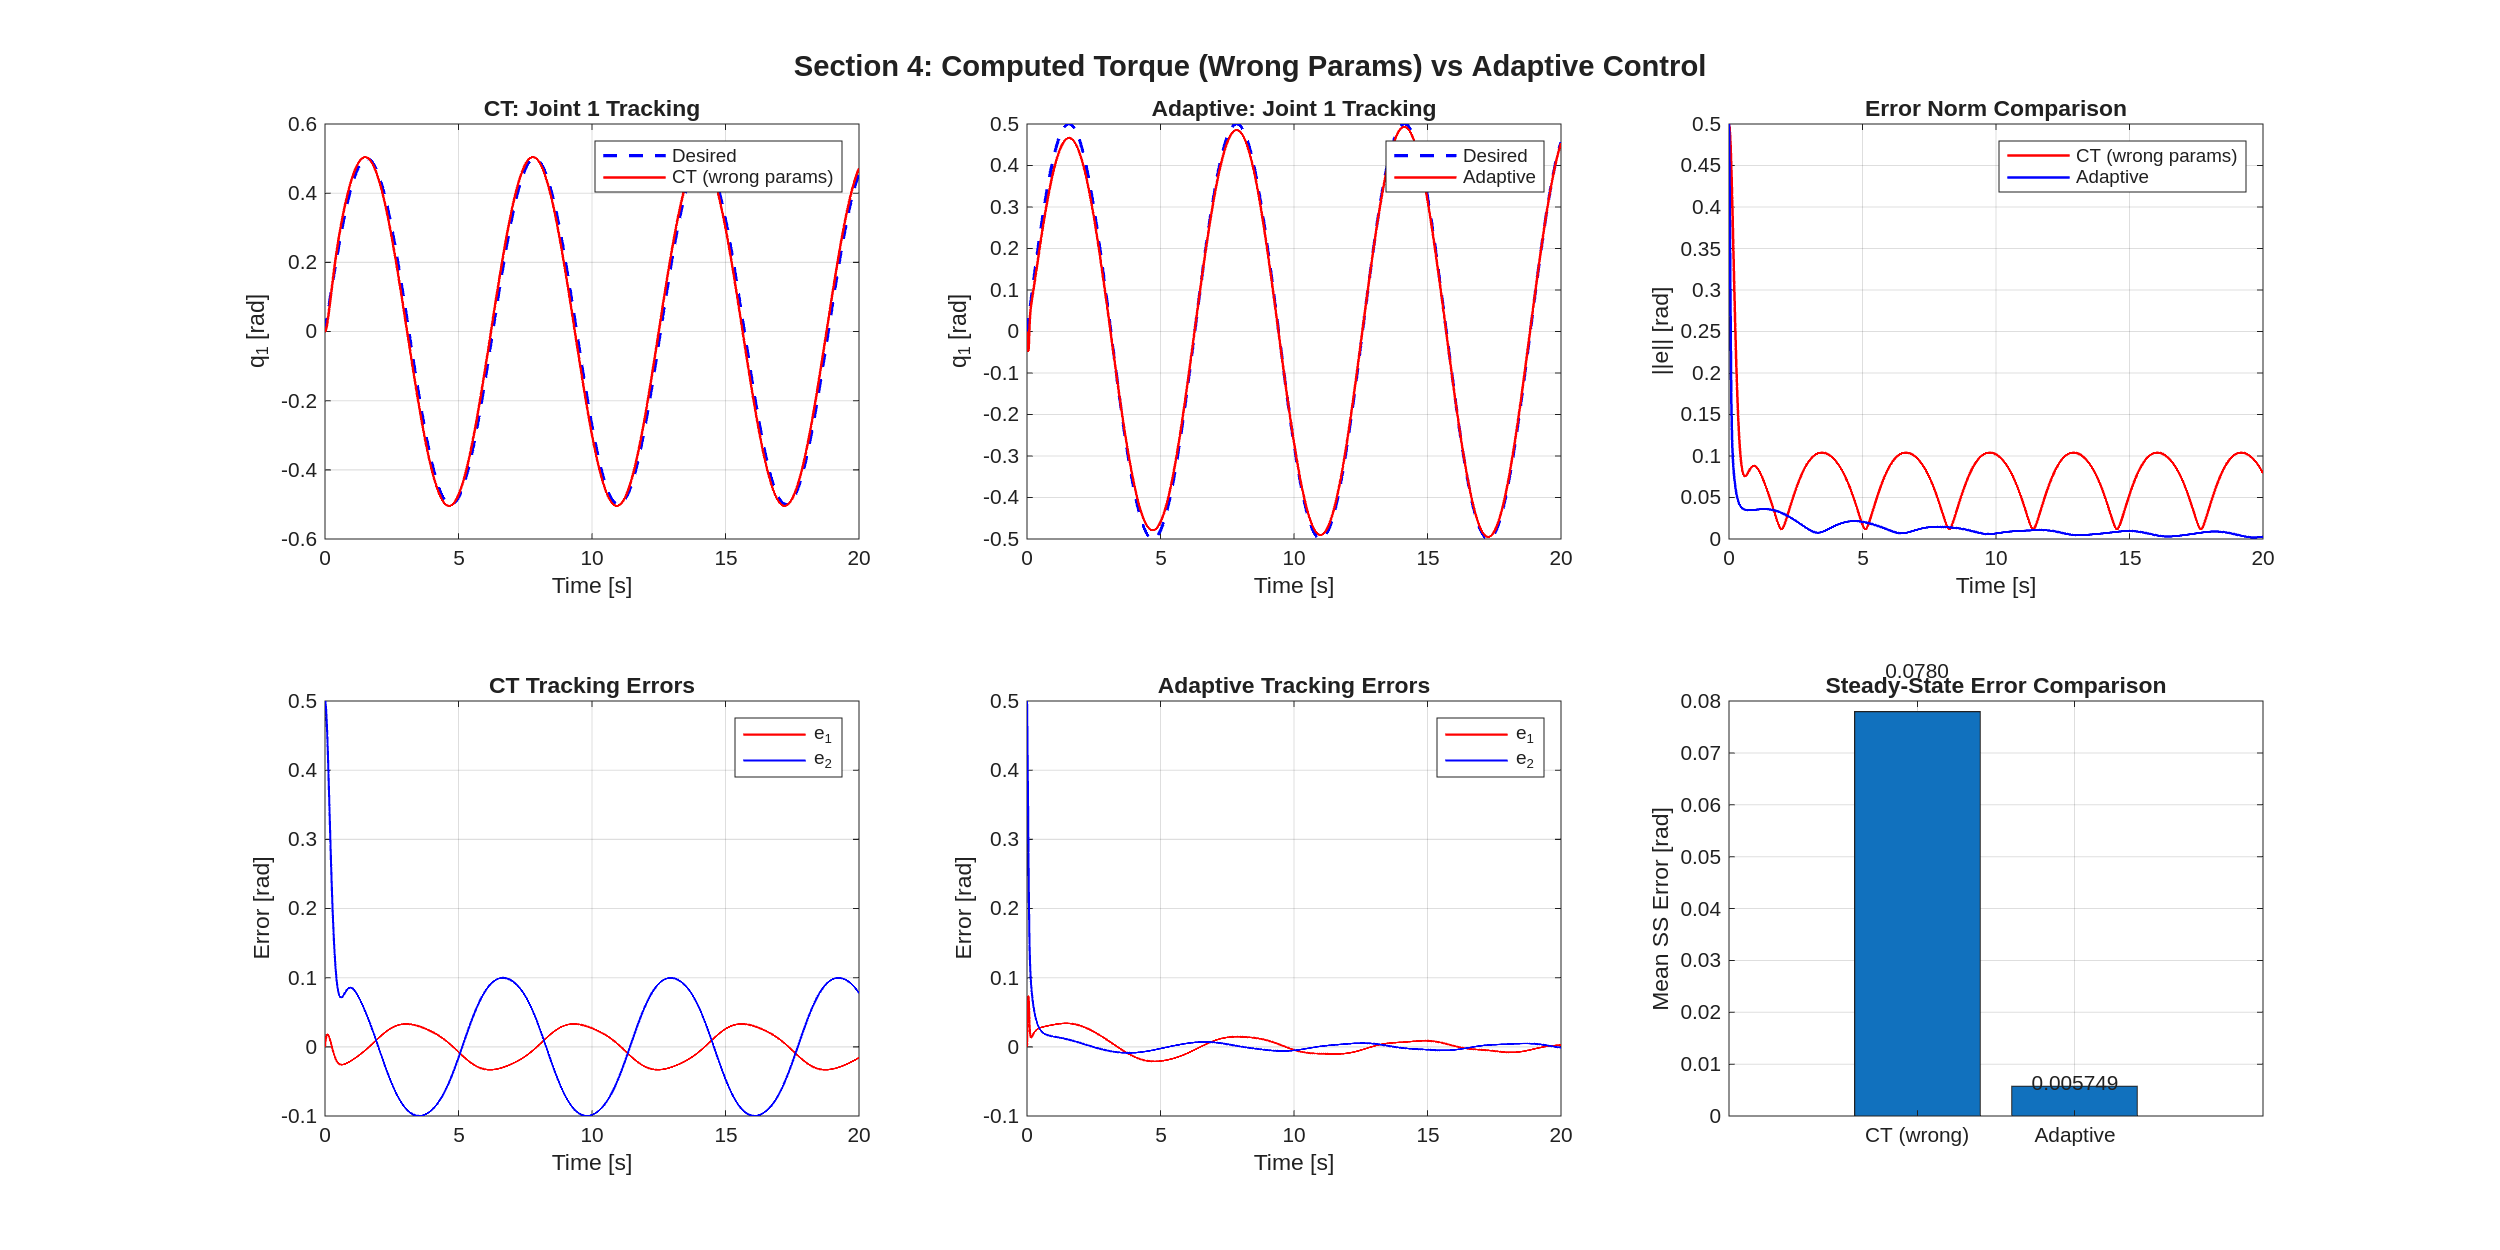
\includegraphics[width=0.92\textwidth,keepaspectratio]{images/week_04/Computed_Torque_vs_Adaptive.png}
    \caption{Computed torque vs adaptive.}
\end{figure}

\begin{figure}[ht]
    \centering
    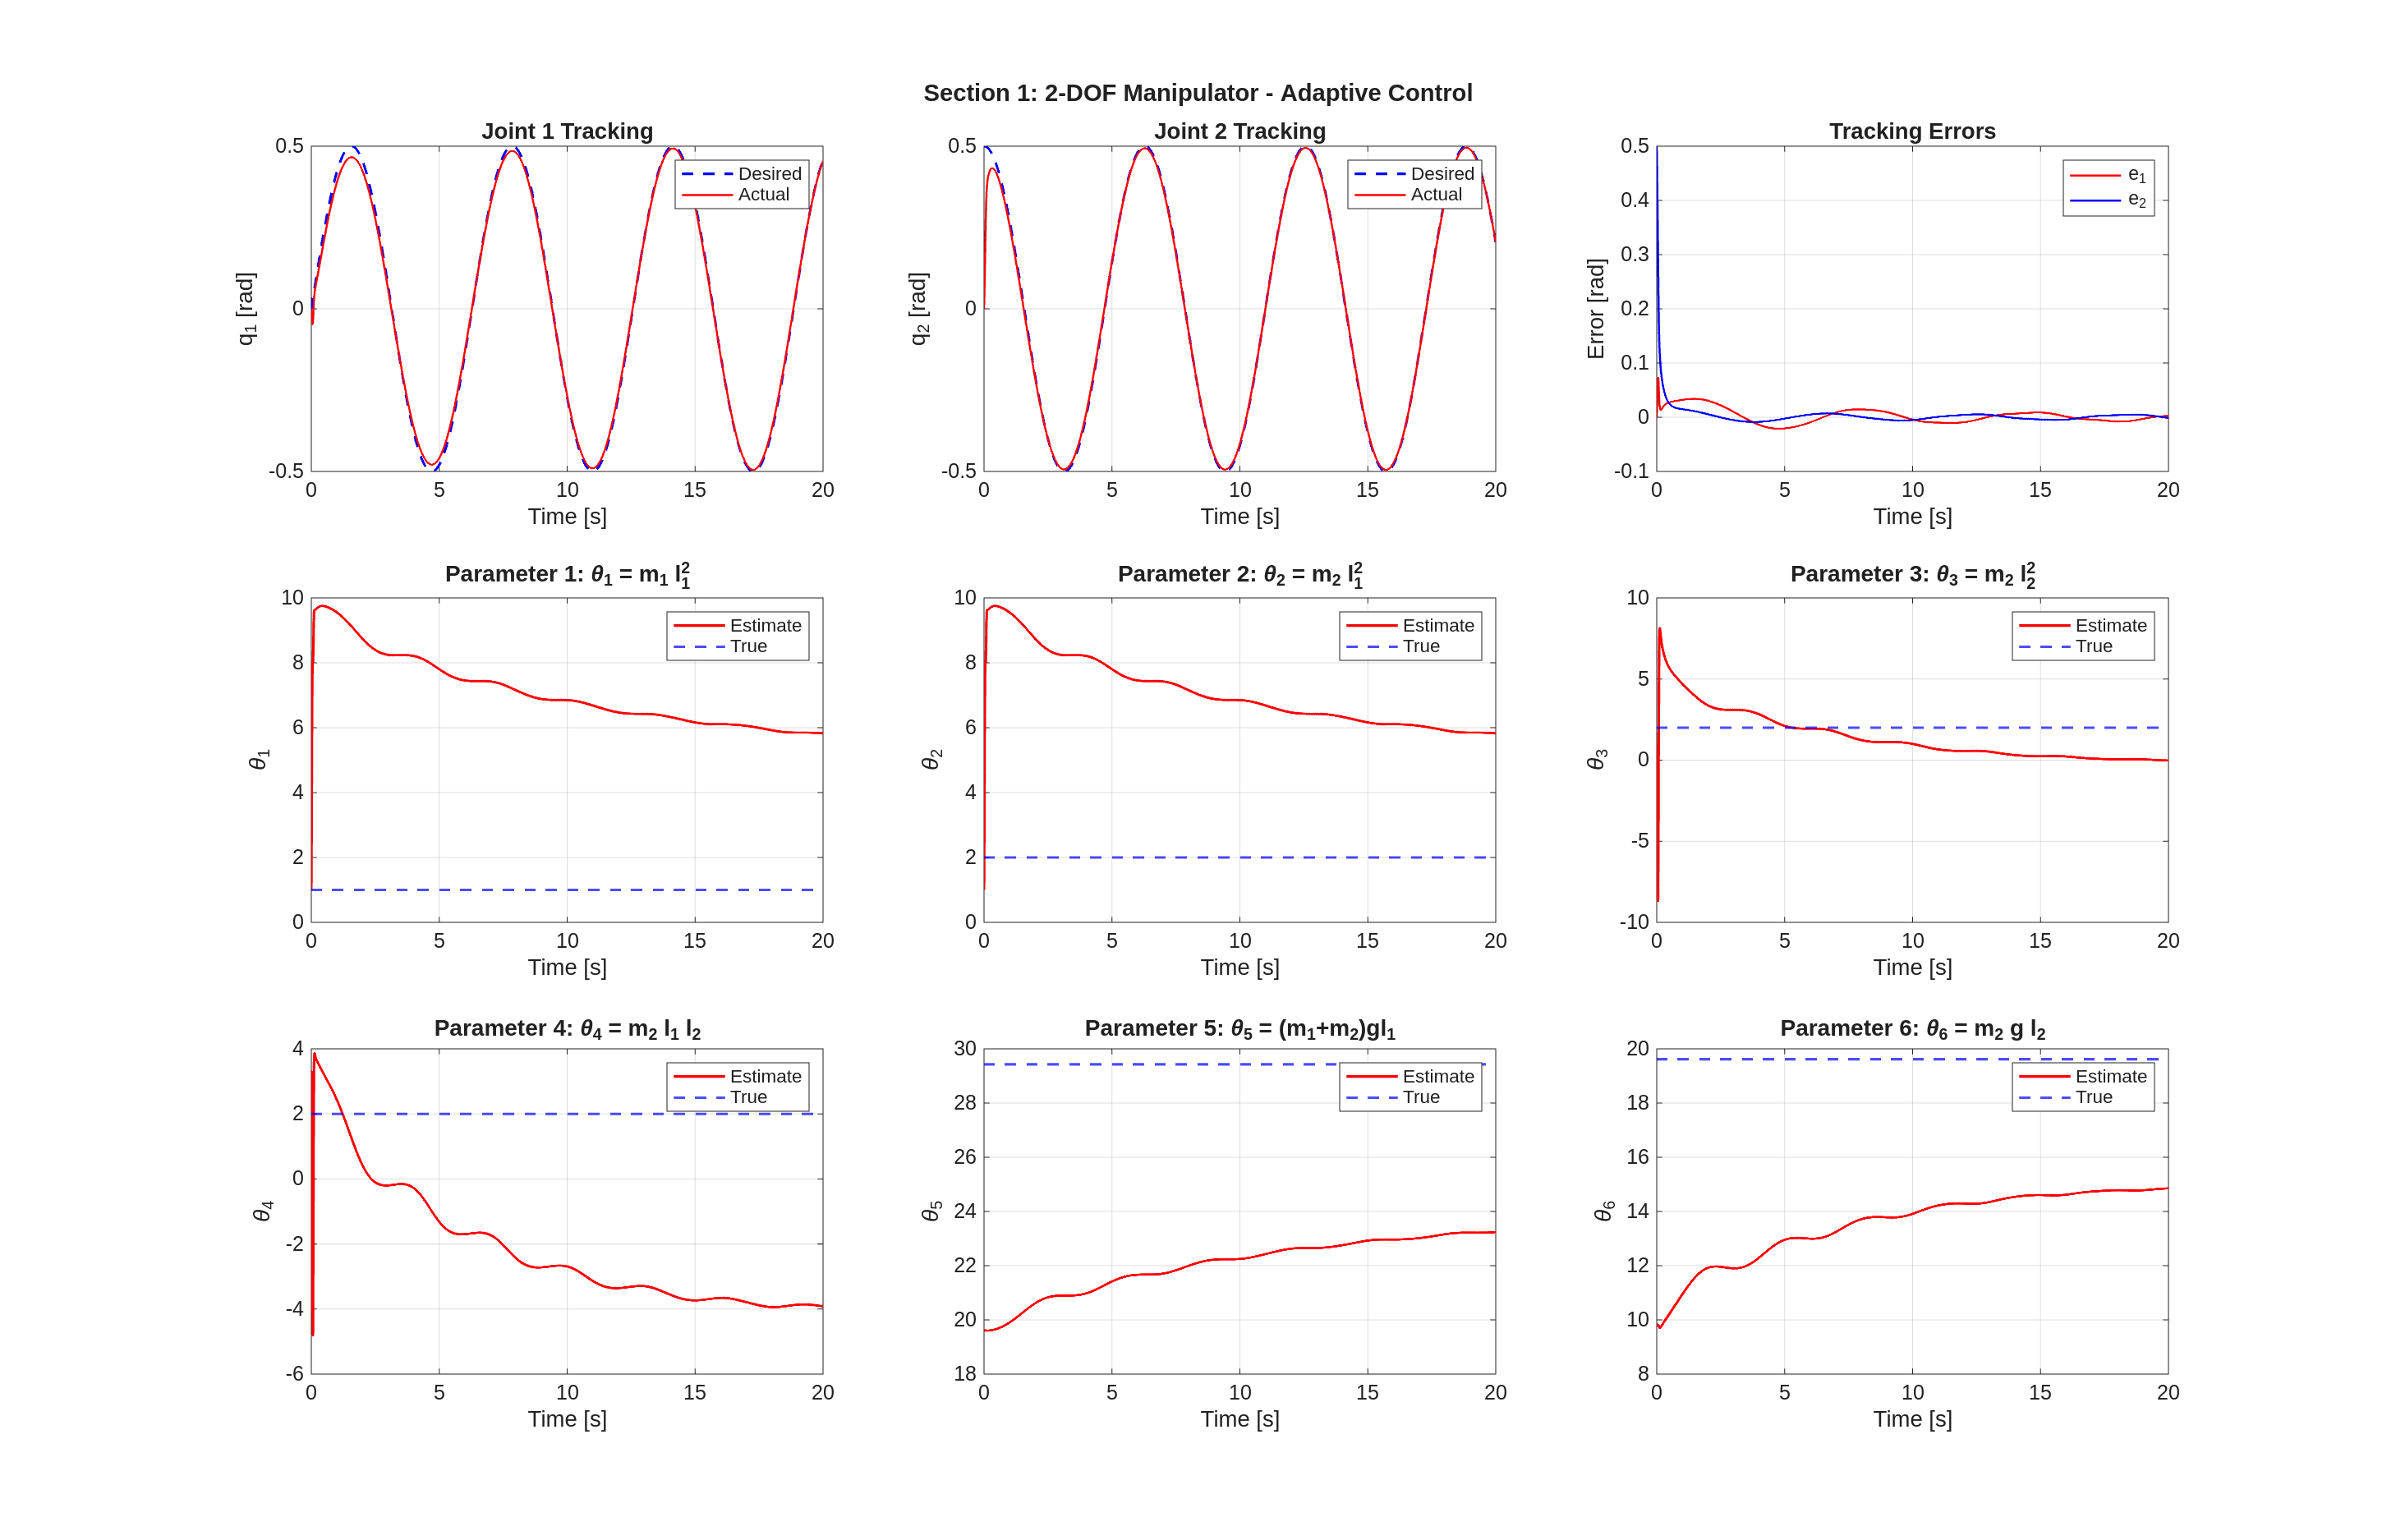
\includegraphics[width=0.92\textwidth,keepaspectratio]{images/week_04/Manipulator_Adaptive_Control.png}
    \caption{Manipulator adaptive control.}
\end{figure}

\begin{figure}[ht]
    \centering
    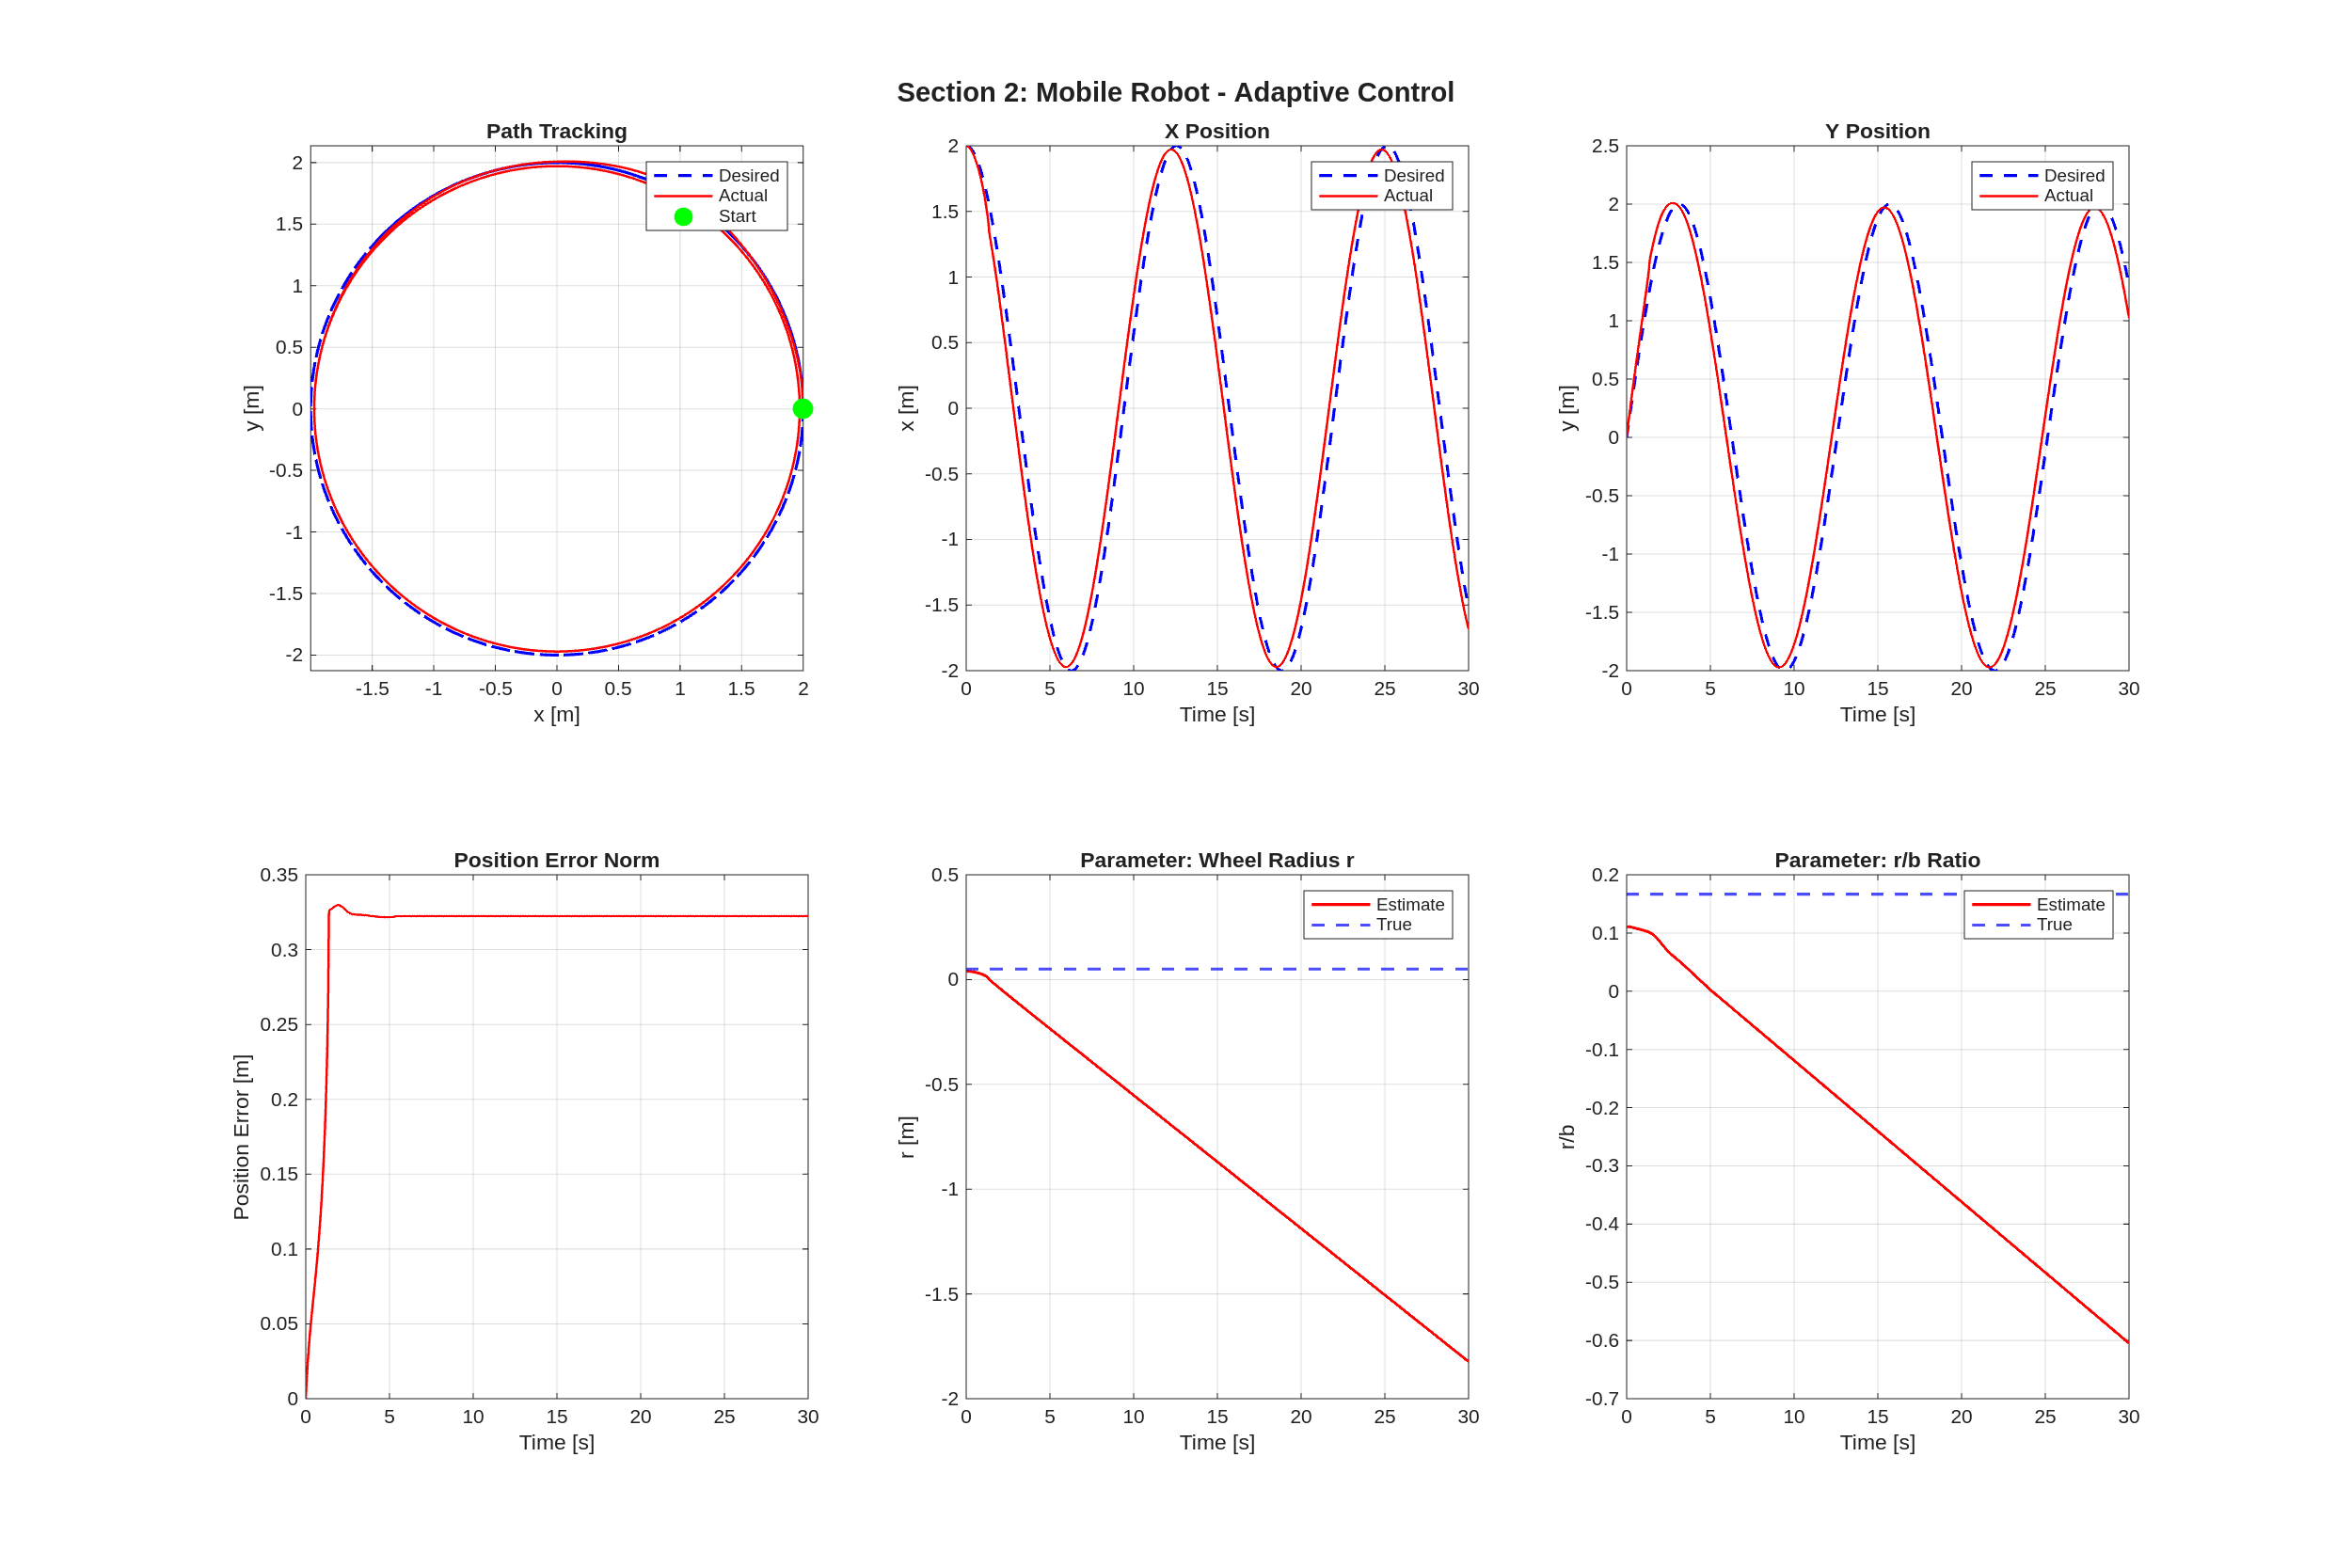
\includegraphics[width=0.92\textwidth,keepaspectratio]{images/week_04/Mobile_Robot_Adaptive_Control.png}
    \caption{Mobile robot adaptive control.}
\end{figure}

\begin{figure}[ht]
    \centering
    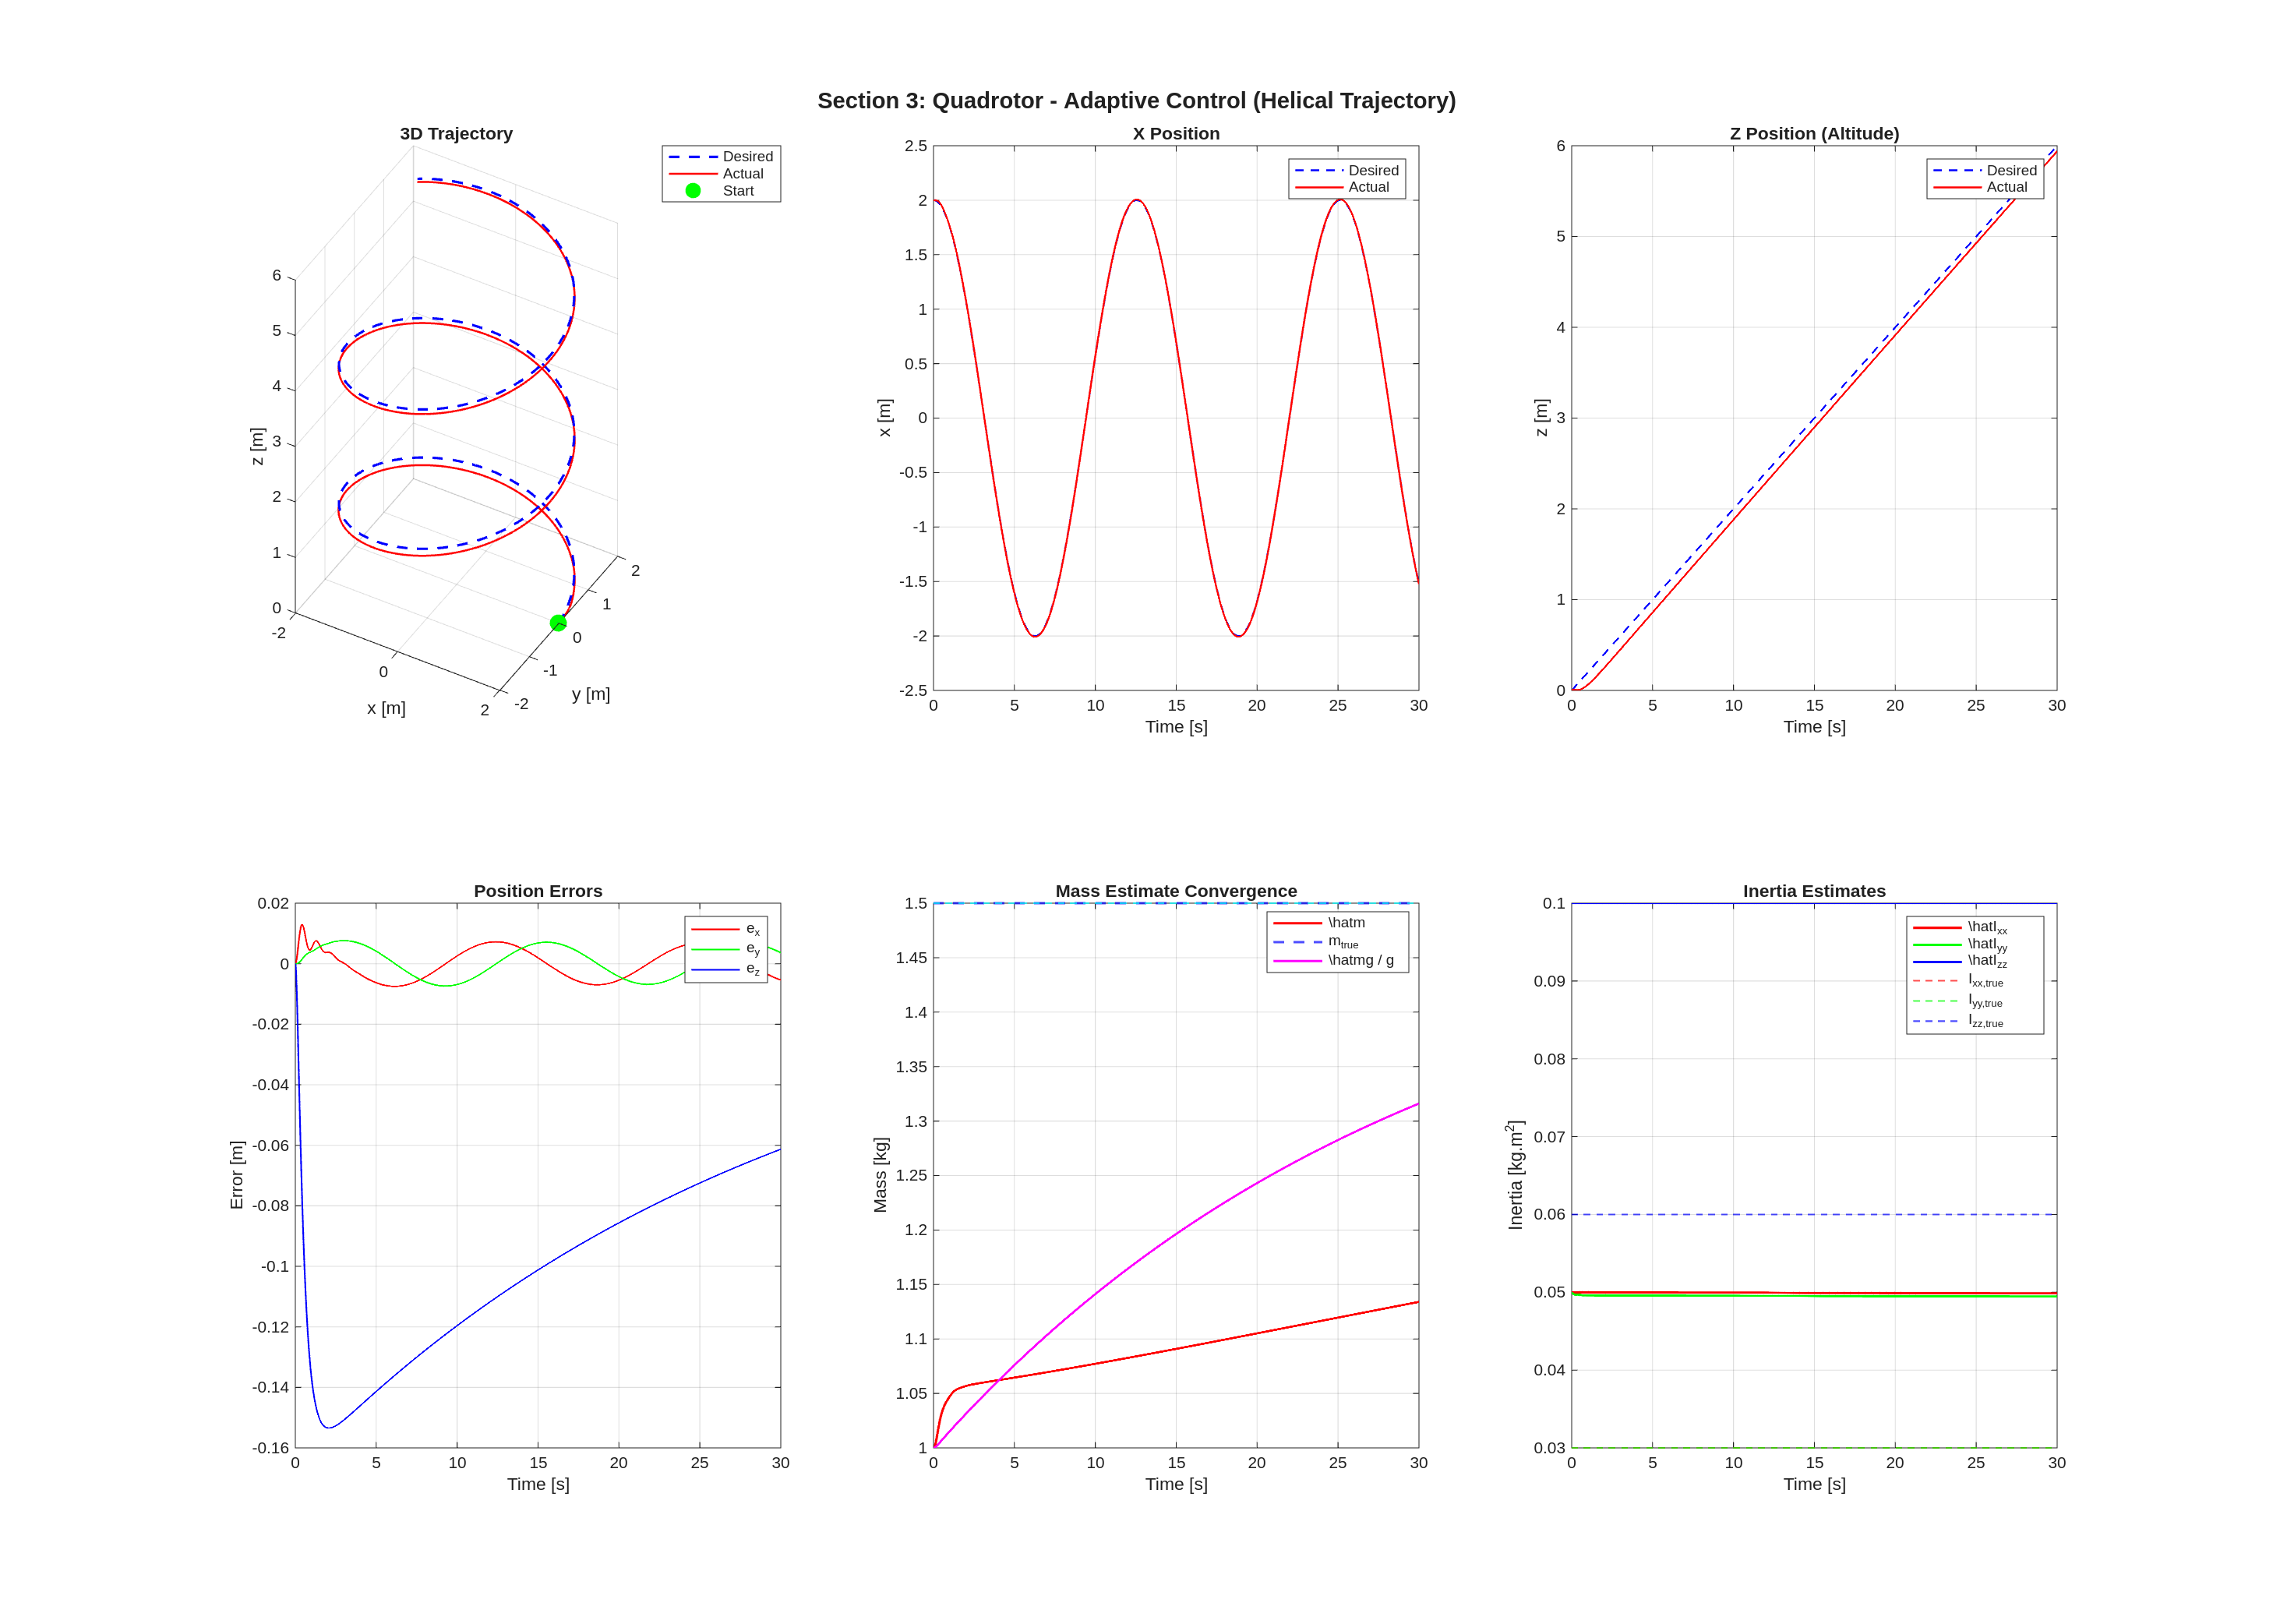
\includegraphics[width=0.92\textwidth,keepaspectratio]{images/week_04/Quadrotor_Adaptive_Control.png}
    \caption{Quadrotor adaptive control.}
\end{figure}

\section{Summary and Next Steps}

\subsection{Summary --- Control Methods Comparison}

\begin{table}[ht]\footnotesize\centering
\adjustbox{max width=\textwidth,max totalheight=0.85\textheight}{%
\begin{tabular}{llll}

\topruleProperty & Computed Torque (Week 1) & MPC (Week 2) & Adaptive Control (Week 3) \\
\midrule\bottomrule\textbf{Core idea} & Cancel nonlinearities with exact model, reduce to linear error dynamics & Predict future states over horizon, optimise control sequence online & Estimate unknown parameters online while controlling; Lyapunov guarantees stability \\
\textbf{Model requirement} & Exact knowledge of \(M(q), C(q,\dot{q}), G(q)\) & Known (possibly linearised) model for prediction & Known structure (regressor \(Y\)), unknown parameter values (\(\theta\)) \\
\textbf{Handles uncertainty?} & No --- performance degrades with parameter errors & Partially --- robust MPC variants exist but add conservatism & Yes --- explicitly designed for parametric uncertainty \\
\textbf{Handles constraints?} & No (must add saturation externally) & Yes --- naturally incorporates state and input constraints & Not directly (parameter projection can enforce bounds on \(\hat{\theta}\)) \\
\textbf{Computation} & Low --- one matrix inversion per step & High --- solves QP at each step & Low --- regressor multiply + parameter ODE integration \\
\textbf{Stability guarantee} & Exponential (with exact model) & Guaranteed with terminal cost/constraint & Asymptotic via Lyapunov + Barbalat\textquotesingle s lemma \\
\textbf{Parameter convergence} & N/A (parameters assumed known) & N/A (parameters assumed known) & Only with persistent excitation \\
\textbf{Key design parameters} & \(K_p, K_v\) (PD gains) & \(Q, R, N\) (cost weights, horizon) & \(\Lambda, K_D, \Gamma\) (sliding surface, damping, adaptation rate) \\
\textbf{Best suited for} & Well-modelled systems with known parameters & Systems with constraints, preview information, and known models & Systems with unknown or slowly-varying parameters, no constraints \\
\end{tabular}}
\end{table}


\textbf{Looking ahead --- Week 4: Robust Control.} What if the uncertainty is not parametric but includes unmodelled dynamics, disturbances, or unstructured uncertainty? Robust control (e.g., sliding mode control, \(H_\infty\)) provides guaranteed performance bounds without requiring online estimation. We will see how robust and adaptive approaches can be combined.

M.Sc. Control for Robots --- AY 2025--26

Week 3: Adaptive Control • Lecture Notes
